\documentclass[11pt]{article}
\usepackage[top=1.5cm,bottom=1.5cm,left=1.5cm,right= 1.5cm]{geometry}
%\geometry{landscape}                % Activate for for rotated page geometry
\usepackage[parfill]{parskip}    % Activate to begin paragraphs with an empty line rather than an indent
\usepackage{graphicx}
\usepackage{amssymb}
\usepackage{epstopdf}
\usepackage{setspace}            
\usepackage{amsmath}            
\usepackage{multirow}    
\usepackage{changepage}
\usepackage{lscape}
\usepackage{ulem}
\usepackage{multicol}
\usepackage{dashrule}
\usepackage[usenames,dvipsnames]{color}       
\usepackage{enumerate}
\newcommand{\urlwofont}[1]{\urlstyle{same}\url{#1}}
\newcommand{\degree}{\ensuremath{^\circ}}

\DeclareGraphicsRule{.tif}{png}{.png}{`convert #1 `dirname #1`/`basename #1 .tif`.png}

\newenvironment{choices}{
\begin{enumerate}[(a)]
}{\end{enumerate}}

\pagestyle{empty}

%\newcommand{\soln}[1]{\textcolor{MidnightBlue}{\textit{#1}}}	% delete #1 to get rid of solutions for handouts
\newcommand{\soln}[1]{ \vspace{2.7cm} }

\newcommand{\solnMult}[1]{\textbf{\textcolor{MidnightBlue}{\textit{#1}}}}	% uncomment for solutions
%\newcommand{\solnMult}[1]{ #1 }	% uncomment for handouts

%\newcommand{\pts}[1]{ \textbf{{\footnotesize \textcolor{black}{(#1)}}} }	% uncomment for handouts
\newcommand{\pts}[1]{ \textbf{{\footnotesize \textcolor{red}{(#1)}}} }	% uncomment for handouts

\newcommand{\note}[1]{ \textbf{\textcolor{red}{[#1]}} }	% uncomment for handouts

\definecolor{oiG}{rgb}{.298,.447,.114}
\definecolor{oiB}{rgb}{.337,.608,.741}

\usepackage[colorlinks=false,pdfborder={0 0 0},urlcolor= oiG,colorlinks=true,linkcolor= oiG, citecolor= oiG,backref=true]{hyperref}

%\usepackage{draftwatermark}
%\SetWatermarkScale{4}

\usepackage{titlesec}
\titleformat{\section}
{\color{oiB}\normalfont\Large\bfseries}
{\color{oiB}\thesection}{1em}{}
\titleformat{\subsection}
{\color{oiB}\normalfont}
{\color{oiB}\thesubsection}{1em}{}

\newcommand{\ttl}[1]{ \textsc{{\LARGE \textbf{{\color{oiB} #1} } }}}

\newcommand{\tl}[1]{ \textsc{{\large \textbf{{\color{oiB} #1} } }}}

\begin{document}

Dr. \c{C}etinkaya-Rundel \hfill Data Analysis and Statistical Inference \\

\ttl{Application exercise: 4.3 ANOVA, Part 2} 

\section*{Teacher evaluations}

Many college courses conclude by giving students the opportunity to evaluate the course and the instructor anonymously. In this application exercise we evaluate whether the teaching evaluations for instructors vary by their rank: teaching, tenure track, and tenured. Note that the instructors are evaluated on a 1-5 scale (1-low, 5-high).

The data come from ``Beauty in the classroom: instructors' pulchritude and putative pedagogical productivity'' (Hamermesh and Parker, 2005) found that instructors who are viewed to be better looking receive higher instructional ratings.\footnote{Daniel S. Hamermesh, Amy Parker, Beauty in the classroom: instructors� pulchritude and putative pedagogical productivity, \textit{Economics of Education Review}, Volume 24, Issue 4, August 2005, Pages 369-376, ISSN 0272-7757, 10.1016/j.econedurev.2004.07.013. (\href{http://www.sciencedirect.com/science/article/pii/S0272775704001165}{http://www.sciencedirect.com/science/article/pii/S0272775704001165}).}, which is a dataset we will work with again later in the course.

\begin{center}
\begin{tabular}{l | c | c | c | c | c | c | c | c}
		& Min. & 1st Qu. & Median  &  Mean & 3rd Qu. &   Max. & Std. Dev. & n \\
\hline
teaching	&  3.300 &  3.900  & 4.400&   4.284 &  4.700&   5.000 	& 0.5 & 102 \\
tenure track	& 2.300 &  3.700 &  4.350  & 4.155 &  4.600  & 4.900 & 0.56 & 108 \\
tenured 	&   2.400   & 3.800 &  4.200  & 4.139  & 4.600 &  5.000  & 0.55 & 253
\end{tabular}
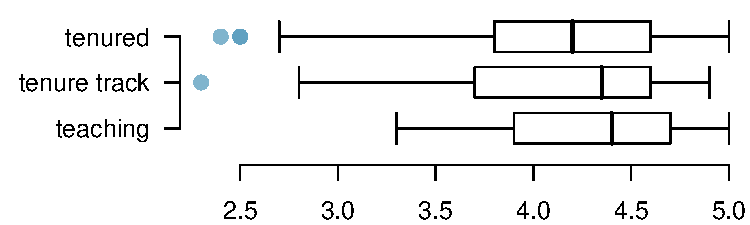
\includegraphics[width=0.6\textwidth]{figures/evals_rank}
\end{center}

%

\begin{enumerate}

\item If the result of the ANOVA from Part 1 is significant, conduct multiple comparisons tests to find out which pairs of means are different.

\item BONUS: Load the dataset and conduct the ANOVA using the inference function. Note that the first variable is the response, and the second variable is the explanatory variable. For the rest of the necessary arguments the function should give you errors that lead you in the right direction. Copy and paste your code + output.

\begin{verbatim}
download("http://stat.duke.edu/~mc301/data/evals.RData", destfile = "evals.RData")
load("evals.RData")
\end{verbatim}

\end{enumerate}

%

\end{document}